%%%%%%%%%%%%%%%%%%%%%%%%%%%%%%%%%%%%%%%%%
% Masters/Doctoral Thesis 
% LaTeX Template
% Version 2.5 (27/8/17)
%
% This template was downloaded from:
% http://www.LaTeXTemplates.com
%
% Version 2.x major modifications by:
% Vel (vel@latextemplates.com)
%
% This template is based on a template by:
% Steve Gunn (http://users.ecs.soton.ac.uk/srg/softwaretools/document/templates/)
% Sunil Patel (http://www.sunilpatel.co.uk/thesis-template/)
%
% Template license:
% CC BY-NC-SA 3.0 (http://creativecommons.org/licenses/by-nc-sa/3.0/)
%
%%%%%%%%%%%%%%%%%%%%%%%%%%%%%%%%%%%%%%%%%

%----------------------------------------------------------------------------------------
%	PACKAGES AND OTHER DOCUMENT CONFIGURATIONS
%----------------------------------------------------------------------------------------

\documentclass[
11pt, % The default document font size, options: 10pt, 11pt, 12pt
%oneside, % Two side (alternating margins) for binding by default, uncomment to switch to one side
italian, % ngerman for German
singlespacing, % Single line spacing, alternatives: onehalfspacing or doublespacing
%draft, % Uncomment to enable draft mode (no pictures, no links, overfull hboxes indicated)
%nolistspacing, % If the document is onehalfspacing or doublespacing, uncomment this to set spacing in lists to single
%liststotoc, % Uncomment to add the list of figures/tables/etc to the table of contents
%toctotoc, % Uncomment to add the main table of contents to the table of contents
%parskip, % Uncomment to add space between paragraphs
%nohyperref, % Uncomment to not load the hyperref package
headsepline, % Uncomment to get a line under the header
%chapterinoneline, % Uncomment to place the chapter title next to the number on one line
%consistentlayout, % Uncomment to change the layout of the declaration, abstract and acknowledgements pages to match the default layout
]{MastersDoctoralThesis} % The class file specifying the document structure

\usepackage[utf8]{inputenc} % Required for inputting international characters
\usepackage[T1]{fontenc} % Output font encoding for international characters

\usepackage{mathpazo} % Use the Palatino font by default

\usepackage[backend=bibtex,style=authoryear,natbib=true]{biblatex} % Use the bibtex backend with the authoryear citation style (which resembles APA)

\addbibresource{example.bib} % The filename of the bibliography

\usepackage[autostyle=true]{csquotes} % Required to generate language-dependent quotes in the bibliography

%----------------------------------------------------------------------------------------
%	MARGIN SETTINGS
%----------------------------------------------------------------------------------------

\geometry{
	paper=a4paper, % Change to letterpaper for US letter
	inner=2.5cm, % Inner margin
	outer=3.8cm, % Outer margin
	bindingoffset=.5cm, % Binding offset
	top=1.5cm, % Top margin
	bottom=1.5cm, % Bottom margin
	%showframe, % Uncomment to show how the type block is set on the page
}

%----------------------------------------------------------------------------------------
%	THESIS INFORMATION
%----------------------------------------------------------------------------------------

\thesistitle{Computer Grafica nella realizzazione di contenuti d'animazione 3D} % Your thesis title, this is used in the title and abstract, print it elsewhere with \ttitle
\supervisor{Prof. Damiana \textsc{Lazzaro}} % Your supervisor's name, this is used in the title page, print it elsewhere with \supname
\examiner{} % Your examiner's name, this is not currently used anywhere in the template, print it elsewhere with \examname
\degree{Laurea} % Your degree name, this is used in the title page and abstract, print it elsewhere with \degreename
\author{Leonardo \textsc{Marini}} % Your name, this is used in the title page and abstract, print it elsewhere with \authorname
\addresses{} % Your address, this is not currently used anywhere in the template, print it elsewhere with \addressname

\subject{Computer Graphics} % Your subject area, this is not currently used anywhere in the template, print it elsewhere with \subjectname
\keywords{tesi, 3D, graphics, cortometraggio, tecniche, animazione} % Keywords for your thesis, this is not currently used anywhere in the template, print it elsewhere with \keywordnames
\university{\href{https://www.unibo.it/it}{Alma Mater Studiorum - Università di Bologna}} % Your university's name and URL, this is used in the title page and abstract, print it elsewhere with \univname
\campus{\href{https://www.unibo.it/it/campus-cesena}{Campus di Cesena}} % Your university's name and URL, this is used in the title page and abstract, print it elsewhere with \univname
\department{\href{https://disi.unibo.it/it}{Dipartimento di Informatica --- Scienza e Ingegneria}} % Your department's name and URL, this is used in the title page and abstract, print it elsewhere with \deptname
\group{\href{http://researchgroup.university.com}{Research Group Name}} % Your research group's name and URL, this is used in the title page, print it elsewhere with \groupname
\faculty{\href{https://corsi.unibo.it/laurea/IngegneriaScienzeInformatiche}{Corso di Laurea in Ingegneria e Scienze Informatiche}} % Your faculty's name and URL, this is used in the title page and abstract, print it elsewhere with \facname

\AtBeginDocument{
\hypersetup{pdftitle=\ttitle} % Set the PDF's title to your title
\hypersetup{pdfauthor=\authorname} % Set the PDF's author to your name
\hypersetup{pdfkeywords=\keywordnames} % Set the PDF's keywords to your keywords
}

\begin{document}

\frontmatter % Use roman page numbering style (i, ii, iii, iv...) for the pre-content pages

\pagestyle{plain} % Default to the plain heading style until the thesis style is called for the body content

%----------------------------------------------------------------------------------------
%	TITLE PAGE
%----------------------------------------------------------------------------------------

\begin{titlepage}
\begin{center}

\vspace*{.06\textheight}
{\scshape\Large \univname\\\large\campname\par}\vspace{1.5cm} % University name
\textsc{\deptname\\\facname}\\ % Thesis type

\vfill
\HRule \\[0.4cm] % Horizontal line
{\huge \bfseries \ttitle\par}\vspace{0.4cm} % Thesis title
\HRule \\[1.5cm] % Horizontal line
 
\vfill
\large {Elaborato in \\\textit{\subjectname}}\\[0.3cm] % University requirement text
\vfill

\begin{minipage}[t]{0.4\textwidth}
\begin{flushleft} \large
\emph{Relatore:}\\
\href{https://www.unibo.it/sitoweb/damiana.lazzaro}{\supname} % Supervisor name - remove the \href bracket to remove the link  
\end{flushleft}
\end{minipage}
\begin{minipage}[t]{0.4\textwidth}
\begin{flushright} \large
\emph{Presentata da:} \\
\href{https://www.linkedin.com/in/leonardo-marini-it/}{\authorname} % Author name - remove the \href bracket to remove the link
\end{flushright}
\end{minipage}\\[3cm]
 
\vfill

{\large Anno Accademico 2019 --- 2020}\\[4cm] % Date
%\includegraphics{Logo} % University/department logo - uncomment to place it
 
\vfill
\end{center}
\end{titlepage}

%----------------------------------------------------------------------------------------
%	ABSTRACT PAGE
%----------------------------------------------------------------------------------------

\renewcommand{\abstractname}{Abstract}
\begin{abstract}
\addchaptertocentry{\abstractname} % Add the abstract to the table of contents
The Thesis Abstract is written here (and usually kept to just this page). The page is kept centered vertically so can expand into the blank space above the title too\ldots
\end{abstract}

%----------------------------------------------------------------------------------------
%	ACKNOWLEDGEMENTS
%----------------------------------------------------------------------------------------

\begin{acknowledgements}
\addchaptertocentry{\acknowledgementname} % Add the acknowledgements to the table of contents
The acknowledgments and the people to thank go here, don't forget to include your project advisor\ldots
\end{acknowledgements}

%----------------------------------------------------------------------------------------
%	LIST OF CONTENTS/FIGURES/TABLES PAGES
%----------------------------------------------------------------------------------------

\tableofcontents % Prints the main table of contents

\listoffigures % Prints the list of figures

\listoftables % Prints the list of tables

%----------------------------------------------------------------------------------------
%	ABBREVIATIONS
%----------------------------------------------------------------------------------------

\begin{abbreviations}{ll} % Include a list of abbreviations (a table of two columns)

\textbf{LAH} & \textbf{L}ist \textbf{A}bbreviations \textbf{H}ere\\
\textbf{WSF} & \textbf{W}hat (it) \textbf{S}tands \textbf{F}or\\

\end{abbreviations}

%----------------------------------------------------------------------------------------
%	PHYSICAL CONSTANTS/OTHER DEFINITIONS
%----------------------------------------------------------------------------------------

\begin{constants}{lr@{${}={}$}l} % The list of physical constants is a three column table

% The \SI{}{} command is provided by the siunitx package, see its documentation for instructions on how to use it

Speed of Light & $c_{0}$ & \SI{2.99792458e8}{\meter\per\second} (exact)\\
%Constant Name & $Symbol$ & $Constant Value$ with units\\

\end{constants}

%----------------------------------------------------------------------------------------
%	SYMBOLS
%----------------------------------------------------------------------------------------

\begin{symbols}{lll} % Include a list of Symbols (a three column table)

$a$ & distance & \si{\meter} \\
$P$ & power & \si{\watt} (\si{\joule\per\second}) \\
%Symbol & Name & Unit \\

\addlinespace % Gap to separate the Roman symbols from the Greek

$\omega$ & angular frequency & \si{\radian} \\

\end{symbols}

%----------------------------------------------------------------------------------------
%	DEDICATION
%----------------------------------------------------------------------------------------

\dedicatory{For/Dedicated to/To my\ldots} 

%----------------------------------------------------------------------------------------
%	THESIS CONTENT - CHAPTERS
%----------------------------------------------------------------------------------------

\mainmatter % Begin numeric (1,2,3...) page numbering

\pagestyle{thesis} % Return the page headers back to the "thesis" style

% Include the chapters of the thesis as separate files from the Chapters folder
% Uncomment the lines as you write the chapters

% Chapter 1

\chapter{Introduzione} % Main chapter title

\label{Chapter1} % For referencing the chapter elsewhere, use \ref{Chapter1} 


% Background, what is known
La computer grafica (CG) gioca un ruolo molto importante nell'ambito delle scienze informatiche. In particolare, negli ultimi anni si è visto un notevole miglioramento nelle tecniche di rendering fino ad arrivare a risultati di foto-realismo nei quali è praticamente impossibile riconoscere se un'immagine sia stata generata artificialmente (CGI), o se si tratti di una foto.
Ovviamente questi progressi non sono limitati alle immagini statiche, anzi, trovano molte più applicazioni in sequenze video, dove queste immagini sono animate. 
Di fatto, i settori che maggiormente fanno uso di CGI sono quello cinematografico e quello videoludico.
\newline

% Aims & Objectives
Quello delle animazioni digitali, è un sotto settore della CG, tuttavia molto ampio. Questa tesi vuole quindi analizzare questo aspetto, in particolare le esistenti tecniche di animazione 3D, e il contesto in cui queste vengono utilizzate. Per quanto riguarda il contesto, come già detto sopra, quelli principali sono due: film e videogiochi.

Da qui deriva la scelta di realizzare un cortometraggio: la differenza principale tra i due settori, per quanto riguarda le animazioni, è che il primo utilizza animazioni \emph{offline}, mentre per il secondo si parla di animazione in \emph{tempo reale}.
Ciò significa che nel primo caso è possibile sapere in anticipo esattamente quali azioni saranno da animare mentre, nel caso dei videogiochi, è l'utente finale a scegliere quali azioni fare ed in che ordine. Ciò rende più difficile progettare le azioni necessarie, che devono quindi essere spezzate in animazioni cicliche e rendere possibile transitare da un'animazione all'altra. Quest'ultimo aspetto complica ulteriormente le animazioni dei videogiochi: è particolarmente difficile transitare da un'animazione all'altra e rendere tale transizione fluida e realistica lo è ancora di più.
Un altro aspetto, che ha favorito la scelta di realizzare un cortometraggio rispetto ad un videogioco, è che, da un punto di vista progettuale, il primo è costituito da poche semplici fasi, contrariamente ai videogiochi che racchiudono anche il \emph{game-design}, ovvero rendere il gioco in sé giocabile. Sintetizzando, le animazioni rappresentano un aspetto molto piccolo nella realizzazione di un videogioco, mentre ricoprono la parte centrale nella realizzazione di film d'animazione.

L'obiettivo di un cortometraggio è quello di raccontare una storia semplice e a se stante che possa quindi essere rappresentata come filmato dalla breve durata.
La creazione di un cortometraggio animato è quindi un processo che coinvolge l'intera pipeline grafica con l'aggiunta dell'ideazione di una storia da raccontare. L'intero processo di produzione può quindi essere suddiviso in 3 fasi principali: \emph{pre-produzione}, \emph{produzione} e \emph{post-produzione} \parencite{roy2014finish}.
\newline

% Spiegazione dettagliata
In questo caso verrà analizzata soltanto la fase di produzione (Capitolo \ref{Chapter5}), a sua volta suddivisa
in modellazione, texturing, rigging, animazione, lighting e rendering. Una descrizione più dettagliata di ogni
sotto-fase verrà fornita nel rispettivo paragrafo.

Tuttavia, prima di illustrare come sia stato realizzato il corto, verranno spiegate le fasi di analisi e
progettazione. Come per ogni progetto infatti, è indispensabile partire da un'attenta analisi (Capitolo \ref{Chapter2}) del problema per capire cosa si vuole realizzare e studiarne la sua fattibilità. Di conseguenza sarà necessario definire una metodologia, a questo proposito viene illustrata la progettazione (Capitolo \ref{Chapter4}), che ha l'obiettivo di studiare \emph{come} il progetto verrà realizzato.
Quest'ultima fase, come già detto, vuole analizzare l'aspetto metodologico del progetto. Per rendere possibile ciò, vengono quindi riportate le varie tecniche di animazione al capitolo precedente (Capitolo \ref{Chapter3}).

In ogni capitolo verrà data un particolare attenzione alla parte relativa alle animazioni. Sono infatti esse, l'oggetto principale di questa tesi, a differenza del corto, che rappresenta il prodotto finale: un'applicazione della teoria che sta dietro ai vari metodi di animazione, in un contesto lavorativo reale. Vorrei quindi sottolineare come questa tesi inverta il ruolo delle animazioni e del corto. Normalmente, le animazioni, ed in particolare i \emph{rig} che permettono di animare un oggetto 3D, sono il mezzo che permette di raggiungere lo scopo (oggetto animato). In questo caso invece, è il corto a diventare un semplice mezzo attraverso il quale è possibile mostrare l'efficacia della di diverse tecniche di animazione.



%% Chapter 2

\chapter{Analisi} % Main chapter title

\label{Chapter2} % For referencing the chapter elsewhere, use \ref{Chapter1} 

\section{Requisiti} \label{req}
L'obiettivo di questo progetto è la realizzare un cortometraggio animato in 3D.
Questo dovrà quindi rappresentare una storia. Non ci sono requisiti su ciò che possiamo rappresentare, quindi si è deciso per una storia di nostra immaginazione, senza aggiunta di particolare realismo.

Per la storia ne è stata scelta una scritta precedentemente da Alberto, il che ci ha permesso di concentrarci sulla realizzazione del corto, senza spendere tempo per l'ideazione della storia. Questa scelta ha quindi introdotto alcuni nuovi requisiti: come la realizzazione dei modelli dei personaggi e degli ambienti rappresentati nella storia, e la fedeltà allo storyboard realizzato dal mio collega.

Cosa più importante: il corto dovrà essere realizzato utilizzando diverse tecniche di animazione, ciascuna adatta al proprio dominio, al fine di mostrarne le diverse caratteristiche, i vantaggi e gli ambiti in qui ha senso utilizzarle.

Come requisito aggiuntivo, non funzionale, abbiamo puntato ad avere animazioni quanto più realistiche possibili. Questo al solo scopo di avere un prodotto finale piacevole da guardare, e poter mostrare con orgoglio.

\section{Vincoli} 
Visti i limiti di tempo, sia per la realizzazione del video, che per poterlo esporre. Abbiamo deciso di proseguire con la realizzazione di un trailer. Ciò non differisce molto da quella che era l'idea iniziale, e soddisfa i requisiti menzionati nella sezione precedente (\ref{req} Requisiti). Questa scelta offre anche il vantaggio di poter affiancare scene temporalmente distanti tra loro, e anche in ordine cronologico non lineare, per mostrare scene topiche in un crescendo di drammaticità.

Inoltre, in questo modo è stato anche eliminato il problema di doppiare i personaggi. Infatti in un trailer, è possibile utilizzare una colonna sonora di sottofondo, al posto dei dialoghi, generalmente per nascondere \emph{spoiler} presenti in ciò che i personaggi dicono.

Infine, un vincolo fondamentale, e alla base di ogni processo di realizzazione di qualsiasi film, è quello di seguire fedelmente lo storyborad, fornito dal direttore artistico, in questo caso sempre Alberto Uras.

\newpage
\section{Organizzazione del lavoro}
Come per ogni progetto, è importante definire una \emph{tabella di marcia} in maniera tale da non dover rifare le cose più volte, e procedere da un passo all'altro con la consapevolezza di sapere a che punto della produzione ci si trova e, attraverso una stima, capire quanto manca al completamento del prodotto.
Il lavoro è stato quindi suddiviso nelle seguenti task:
\begin{itemize}
    \item Realizzazione e posizione delle scene principali, come key-frame fissi.
    \item Creazione di cicli di animazione da utilizzare in diverse scene.
    \item Implementazione delle animazioni cicliche nelle scene che ne necessitano.
    \item Aggiunta di frame \emph{in-between} e correzione dei movimenti.
    \item Animazione dei dialoghi:
    \begin{itemize}
        \item Creazione delle shape-keys per le diverse espressioni facciali.
        \item Alternare le schape-keys per adattarle all'audio del dialogo.
        \item Aggiunta delle animazioni facciali alle scene animate.
    \end{itemize}
\end{itemize}
 
%% Chapter 3

\chapter{Tecniche di animazione} % Design

\label{Chapter3} % For referencing this chapter elsewhere, use \ref{ChapterX}

Animare significa ``muovere" un modello, altrimenti statico, nel tempo. Questi movimenti sono definiti attraverso delle trasformazioni geometriche (traslazione, rotazione e scalatura).
Di seguito vengono riportate alcune tecniche di animazione 3D, spiegandone le metodologie, i pregi, i difetti e il contesto in cui possono venire utilizzate. 


\section{Rappresentazioni di rotazione}\label{Section3.1}
Iniziamo spigando come si possa rappresentare una rotazione. Alcuni di questi concetti sono validi anche per altre trasformazioni, tuttavia verranno considerate soltanto le rotazioni, in quanto queste ultime sono uno degli aspetti principali nella realizzazione di animazioni --- in particolare di animazioni 3D --- e alla base di alcune tecniche di animazione --- \emph{Inverse Kinematics} (IK) --- come anche uno dei più complessi. 

Come vedremo in seguito sarà indispensabile capire quale delle seguenti rappresentazioni conviene utilizzare in base all'animazione che si vuole realizzare.


\subsection{Angolo-asse}
Questo tipo di rappresentazione è senza dubbio la più semplice.
Utilizza 4 valori: 3 per specificare l'asse, ed 1 per l'angolo. In questo modo, con una singola rotazione, è possibile raggiungere qualsiasi orientamento dell'oggetto che si sta ruotando. Così come esiste sempre una linea retta che collega due punti nello spazio, si può pensare ad una rotazione angolo-asse come una singola rotazione che collega due orientamenti.

Questa rappresentazione, è ottima per rotazioni di articolazioni con un solo \emph{Degree Of Freedom} (DOF). È anche possibile definire articolazioni con più di un DOF semplicemente concatenando $n$ articolazioni su singolo asse connesse da $n-1$ ossa (i.e. oggetti connessi in un'articolazione) di lunghezza 0. Ciò però rende la risultante giuntura inutilmente complessa da animare. Per questo motivo le rappresentazione con angoli di Eulero, o sotto forma di quaternione, sono quelle più spesso utilizzate. Inoltre la rappresentazione dell'asse attraverso 3 componenti numeriche non risulta di facile comprensione per l'utente che di solito preferisce usare quella Euleriana anche per rotazioni su singolo asse.

\subsection{Euleriana}

\begin{figure}
\centering
\begin{subfigure}{.5\textwidth}
  \centering
  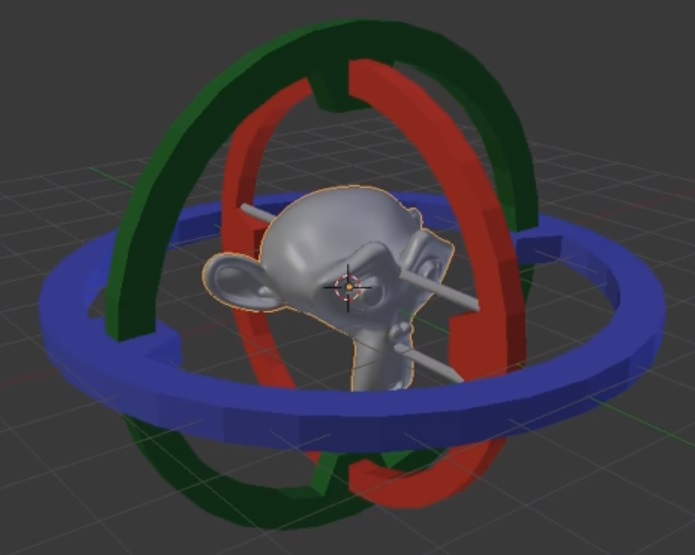
\includegraphics[width=.9\linewidth]{Figures/euler-1.jpg}
  \caption{Posizione neutra.}
  \label{fig:eulerA}
\end{subfigure}%
\begin{subfigure}{.5\textwidth}
  \centering
  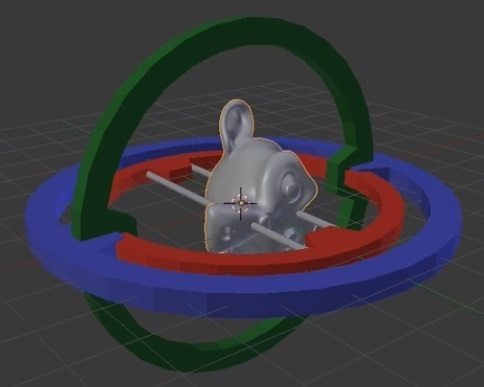
\includegraphics[width=.9\linewidth]{Figures/euler-2.jpg}
  \caption{Gimbal lock, l'asse X e Z sono allineati.}
  \label{fig:eulerB}
\end{subfigure}
\decoRule
\caption[Rotazione Euleriana]{Rappresentazione di rotazione Euleriana attraverso un giroscopio a tre assi.}
  \begin{minipage}{.8\textwidth}
  \footnotesize
  \emph{(Immagine di Nathan Vegdahl)}
  \end{minipage}
\label{fig:euler}
\end{figure}

Concettualmente è la più intuitiva di tutte: utilizza 3 assi di rotazione (X, Y, Z) ed il funzionamento è analogo a quello di un giroscopio. ogni asse offre un DOF, quindi sono possibili rotazioni con 3 DOF. Tuttavia sono necessarie due accortezze: 
\begin{enumerate}
    \item ordine degli assi;
    \item gimbal lock problem.
\end{enumerate}
L'ordine degli assi è decisivo, in quanto quello più interno dipende dalla rotazione di quelli esterni. Di conseguenza ruotando gli assi in un ordine diverso da quello specificato porta a risultati diversi da quello atteso. In più, interpolazioni tra diversi orientamenti, possono a loro volta risultare sgradevoli, poiché la rotazione viene spezzata in 3 movimenti.

Il problema del gimbal lock \parencite{anticz16}, in italiano blocco cardanico, sorge dall'allineamento di due assi: quello più interno e quello più esterno. Ne deriva che ruotano uno di questi 2 assi si ottiene la stessa rotazione, perdendo quindi un DOF.
È quindi importante scegliere l'ordine degli assi in maniera tale che il primo e il terzo non risultino mai allineati.

Per ovviare a questo problema può essere conveniente bloccare uno degli assi in una posizione fissa. Per questo motivo, la forma Euleriana è meglio utilizzata nelle giunture con 1 o 2 DOF.

\subsection{Quaternione}
\begin{figure}[ht]
\centering
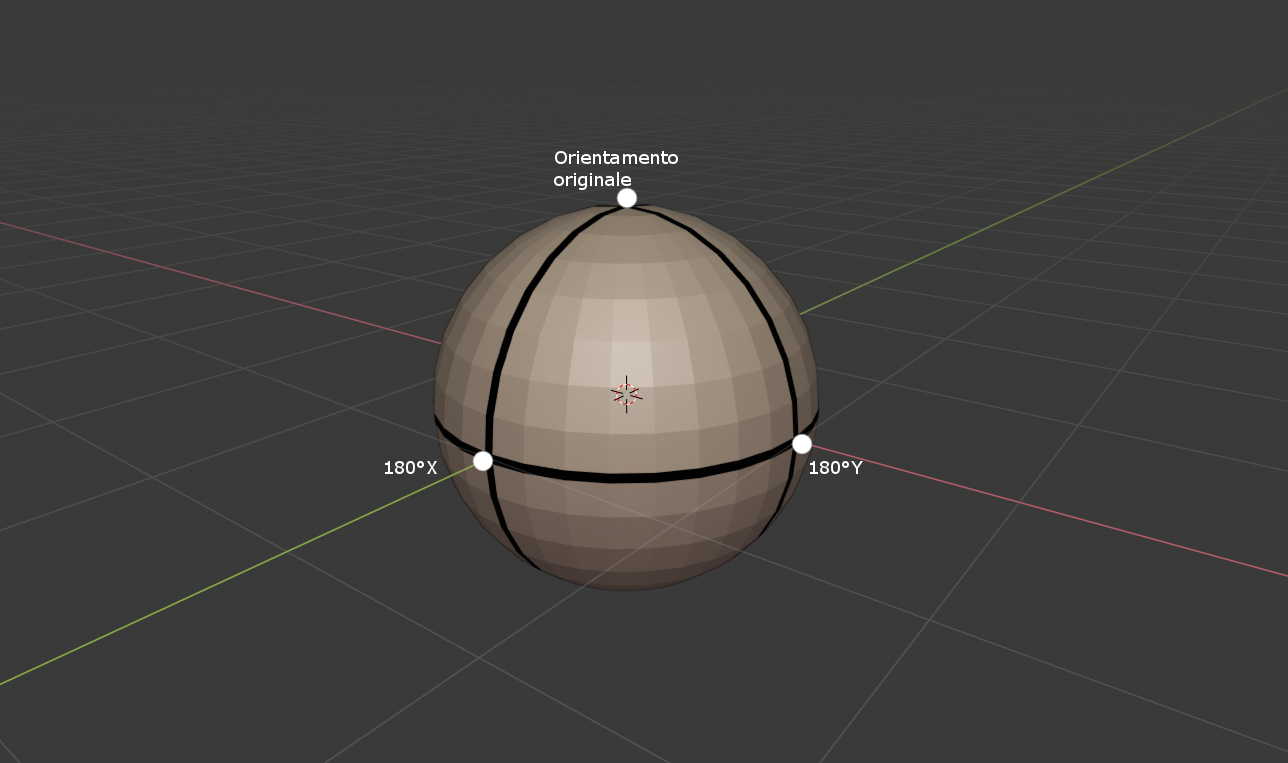
\includegraphics[width=.8\textwidth]{Figures/3d-sphere}
\decoRule
\caption[Quaternione 2D]{Rappresentazione di un quaternione 2D su una sfera 3D.}
\label{fig:quater}
\end{figure}
In contrasto a quanto appena visto, la forma di quaternione è concettualmente complessa, ma in pratica diventa molto utile e senza molti dei difetti della controparte Euleriana.

I principali benefici della rappresentazione a quaternione includono l'eliminazione del gimbal lock. Infatti è presente una componente in più, ma ciascuna componente non rappresenta un asse quanto piuttosto l'orientamento dell'oggetto ruotato intorno a quell'asse. La quarta componente serve quindi a definire la posizione neutra.

L'interpolazione risulta diretta e dolce, infatti il movimento non è spezzato sui diversi assi e l'ordine di questi non è importante. Infine rende comodo calcolare una rotazione opposta semplicememte invertendo il segno della componente W.

Per rendere tutto ciò possibile servono 4 componenti (X, Y, Z, W), come già detto in precedenza, uno per la posizione originale più una per la rotazione su ogni asse. Se si prende il caso di rotazioni su due assi si può immaginare che queste 3 componenti siano 3 punti su una sfera, come mostrato in Figura \ref{fig:quater}. Ogni altra rotazione è data dall'interpolazione di questi tre punti.

La ragione per cui i due punti sulla sfera rappresentano una rotazione di 180\textdegree\ anziché 90\textdegree\ e resa necessaria siccome altrimenti questi due punti coinciderebbero nel punto più basso della sfera. Come effetto aggiuntivo possiamo rappresentare rotazioni fino a 720\textdegree\ ed ogni orientamento equivale a due possibili rotazioni dando all'animatora l'abilità di decidere in che verso ruotare l'oggetto durante un'animazione. 

\subsection{Matriciale}
Quest'ultima è probabilmente la rappresentazione più ottimale in termini di flessibilità, in quanto permette di rappresentare anche traslazioni, scalature e altre trasformazioni come \emph{shear}. È, infatti, la rappresentazione che blender utilizza internamente \cite{blendApi} \cite{nat2012rig} proprio perché offre la maggior flessibilità.

Siccome permette di rappresentare qualsiasi tipo di trasformazione, questa struttura viene solitamente chiamata \emph{Matrice di Trasformazione}. Nel caso di uno spazio a 3 dimensioni, essa ha dimensione $4\times4$.

Questa sua caratteristica la rende indispensabile per rappresentare articolazioni formate da più ossa (i.e Kinematics Linkages) che verranno illustrati qui di seguito (sezioni \ref{sectionFK} e \ref{sectionIK}), poiché rende possibile convertire le coordinate locali di un osso (rappresentato in Figura \ref{fig:FK}, evidenziato in azzurro) figlio a quelle locali del suo padre, fino ad arrivare alle coordinate globali.

L'unico difetto è che, come la rappresentazione sotto forma di quaternione, non mantiene l'informazione sul percorso della rotazione. Infatti è ancora più simile a una delta-rotazione (i.e. differenza di orientamento), rispetto ad un quaternione poiché copre una rotazione di soli 360\textdegree, rispetto ai 720\textdegree\ del quaternione. 

\newpage
\section{Forward Kinematics} \label{sectionFK}

\begin{figure}
\centering
\begin{subfigure}{.33\textwidth}
  \centering
  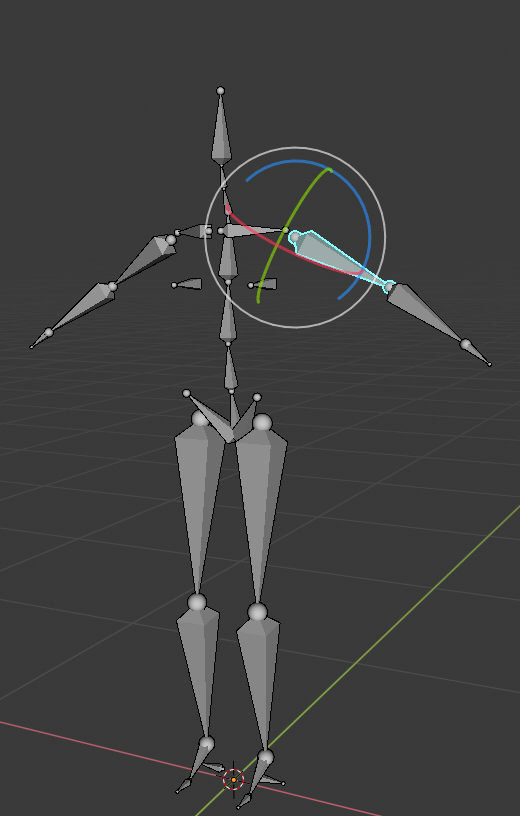
\includegraphics[width=\linewidth]{Figures/armature1}
  \label{fig:FK1}
\end{subfigure}%
\begin{subfigure}{.33\textwidth}
  \centering
  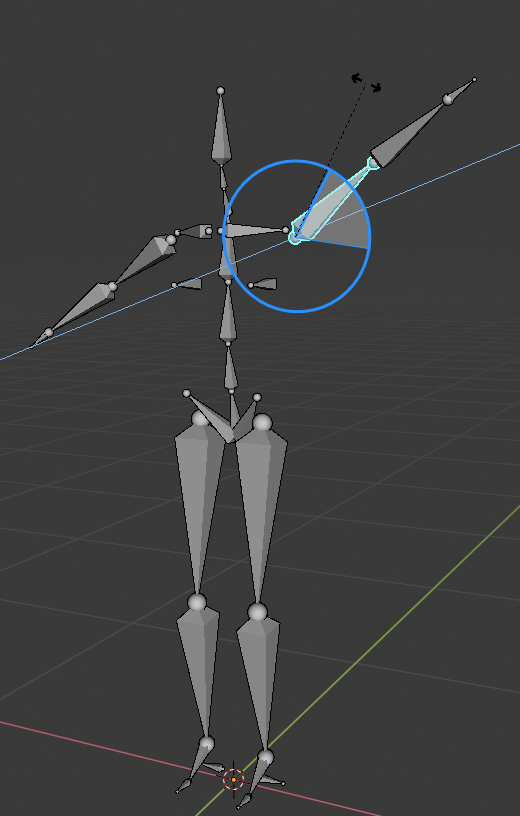
\includegraphics[width=\linewidth]{Figures/armature2}
  \label{fig:FK1}
\end{subfigure}%
\begin{subfigure}{.33\textwidth}
  \centering
  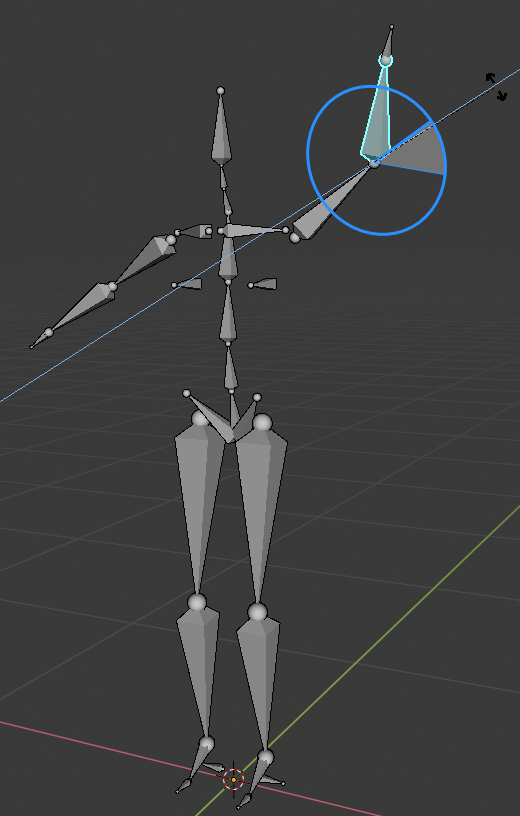
\includegraphics[width=\linewidth]{Figures/armature3}
  \label{fig:FK3}
\end{subfigure}
\decoRule
\caption[Forward Kinematic]{Esempio di posizionamento tramite Forward Kinematic. La figura rappresenta la stessa armatura, formata da diverse ossa, in tre posizioni differenti.}
\label{fig:FK}
\end{figure}

Per figure complesse, come quella umana (da qui in avanti tutti gli esempi saranno riferiti alla figura umana, siccome, nella realizzazione del corto, è stata il centro della maggior parte delle animazioni), è utile avere un sistema che permetta di posizionare le sue componenti in maniera relativa ad altre. Per esempio, una volta posizionato il busto, posizionare il braccio, poi la mano ed in fine le dita, tutto in maniera relativa a quanto posizionato in precedenza.

Questa tecnica permette infatti di specificare, attraverso una rotazione, la posizione di un osso relativa al suo osso padre. Per questo motivo serve che le ossa di un'armatura (vedi Figura \ref{fig:FK}) siano organizzate in maniera gerarchica (i.e. ad albero). In questo modo, quando l'armatura viene posizionata basterà moltiplicare tutte le matrici di trasformazione dalla radice ai nodi foglia in maniera \emph{deep-first}. 
Per definire una posa è quindi necessario specificare la rotazione di ogni osso. Questo permette un controllo preciso su ogni DOF dell'armatura, il che è ottimo, perché permette all'animatore di realizzare pose perfette, senza lasciare che nulla venga calcolato automaticamente. 

Lo svantaggio è che questa metodologia rende difficile animare azioni comuni in cui gli arti si muovono in uno spazio non relativo al resto del corpo, ma rispetto allo spazio circostante. Ad esempio, per aprire una porta tenendo la mano sulla maniglia, il corpo si può spostare di lato, ma la mano deve rimanere aggrappata alla maniglia. Con una metodologia FK, l'animatore dovrebbe infatti spostare il corpo e, ogni volta, riposizionare la mano sulla maniglia, introducendo un sacco di \emph{counter-animation}, ovvero l'animazione inversa per riposizionare la mano nella posizione in cui era prima del movimento del resto del corpo.

\section{Inverse Kinematics} \label{sectionIK}
Definite la posizione della mano e della radice (spalla) la posizione delle ossa intermedie viene calcolata da un algoritmo (e.g. the Jacobian \cite{Parent:2012:CAA:2385444} e iTaSC \cite{blendWiki}).

A volte non esiste nessuna soluzione (mano troppo lontana dalla spalla) e il risultato dev'essere approssimato.

Peggio è se esiste più di una soluzione (undercostrained problem, molto probabile). In tal caso il risultato è scelto dall'algoritmo da una delle possibili soluzioni. Non sempre però tutte sono realistiche o visivamente gradevoli.

È possibile aggiungere dei vincoli per limitare il numero di soluzioni possibili, molto utili quelli per l'imitare il movimento di un arto per renderlo più realistico.
\section{Modularizzare l'animazione}
\subsection{Cicli di animazione}
Il miglior modo per modulare un animazione, ovvero spezzarla in più azioni ripetibili, è quello di individuare le animazioni più frequenti (e.g. camminata, corsa) e definirle una sola volta.
Alcune animazioni, infatti, seguono dei pattern ben definiti.
Grazie alla loro uniformità è possibile renderle cicliche in maniera tale da non dover rifare la stessa animazione più volte.
\subsection{Shape keys}
\subsection{Drivers}
\subsection{Vincoli sulle azioni}
uno dei vantaggi dei vincoli sulle azioni è che è possibile animare le ossa vincolate direttamente, senza aggiungere un osso padre.

Solitamente utilizzate per controllare animazioni molto complesse, come la fuoriuscita del carrello di un aereo al momento dell'atterraggio, attraverso un solo controllo.

%% Chapter 4

\chapter{Progettazione} % Main chapter title

\label{Chapter4} % Change X to a consecutive number; for referencing this chapter elsewhere, use \ref{ChapterX}

Così come nella progettazione di un software si passa dall'analisi alla sua progettazione, prima di svilupparlo. Anche in questo caso, è opportuno progettare l'intero cortometraggio, prima di realizzarlo.
Questo è un passaggio importante poiché non solo permette di capire come il prodotto dovrà essere realizzato, ma permette anche di stabilire delle convenzioni standard (e.g. nomi dei file) da mantenere durante il progetto.
Quest'ultimo aspetto è indispensabile soprattutto nel caso in cui ci siano più persone a lavorare allo stesso progetto.

%----------------------------------------------------------------------------------------
%	SECTION 1
%----------------------------------------------------------------------------------------

\section{Progettazione generale}

%finish your film "Design"
Normalmente la fase di progettazione di un cortometraggio serve a definire l'aspetto dei personaggi e dell'ambientazione (i.e. Character Design, Environment/Prop Design).
Tuttavia questi aspetti sono stati prevalentemente coperti da A. Uras, in quanto il corto rappresenta una storia di sua creazione, e non verranno trattati. La progettazione delle animazioni verrà invece trattata dettagliatamente, in quanto oggetto principale del mio lavoro.

A questo punto del progetto era chiaro che l'obiettivo finale era quello di realizzare un breve trailer di una possibile serie piuttosto che un cortometraggio.
Si è quindi proceduti a selezionare le scene da realizzare per stare entro i due minuti di tempo di riproduzione.

Fatto ciò ho proceduto col creare un flusso di lavoro, in maniera tale da procedere in modo organizzato.
Siccome non ero il solo a lavorare a questo progetto ho scelto un approccio orientato alla produzione, ovvero in cui diversi team si occupano di diversi aspetti del progetto ma che, ciò non di meno, sono collegati e dipendono gli uni dagli altri.

Ad esempio, una volta realizzato il rig base per un modello dev'essere possibile animarlo direttamente, anche senza avere il rig avanzato finale. Ancora più importante è che sia possibile aggiungere dettagli ad un modello, come materiali e textures, anche dopo che questo è stato animato.
Per fare ciò, ho seguito una semplice filosofia: creare l'oggetto una volta e linkarlo in diverse scene invece che copiarlo.
Questa procedura è analoga a quella di utilizzare delle interfacce nella programmazione ad oggetti invece che le classi direttamente. In questo modo, è possibile modificare una classe in un secondo tempo senza alterarne il suo comportamento e, di conseguenza, chi la utilizza non nota alcuna differenza.

Ciò è stato possibile anche grazie alla caratteristica delle armature (o scheletro), di poter essere animate anche quando linkate da un altro file.
In pratica, è possibile definire un proxy che permette di accedere a tutte le proprietà di un'armatura come se questa fosse l'oggetto originale e non una copia (o meglio un link).

\section{Progettazione delle animazioni}

Quando si tratta di sviluppare qualcosa di complesso come una figura umana, è opportuno progettarla, per trovare un modello di astrazione che la semplifichi, pur mantenendo le proprietà che ci interessano e quindi ci permetta di animarla in maniera efficiente.
Il corpo umano è infatti composto da circa duecento DOF \cite{Parent:2012:CAA:2385444}.
Nonostante ciò, la struttura esteriore è fondamentalmente composta da un'unica mesh.
Quindi, rispetto a quanto visto fin'ora, dove la struttura da animare era un'armatura composta da più ossa, sarà necessario deformare la mesh per adattarla all'armatura sottostante. Ciò è possibile associando determinati vertici della mesh ad ogni osso.

La progettazione del rig (Figura \ref{fig:rig}) serve ad ottenere una serie di controlli interattivi mirati a facilitare l'animazione del personaggio.
L'usabilità di un rig è un aspetto fondamentale, in quanto, se il rig non è semplice da utilizzare per un animatore, esso è completamente inutile.
Il rig, infatti, non è fine a se stesso, ma è lo strumento che permettera (solitamente ad altri) di animare i nostri modelli.
La progettazione delle animazione consiste dunque nell'ideare un rig che ci permetterà poi di animare i medelli efficientemente. Parlare di progettazione di animazioni o di rig è quindi indifferente.
Per progettare un buon rig serve, prima di tutto, individuarne l'obiettivo, per rendere il rig il più semplice possibile.
Di seguito sono riportati alcuni degli obiettivi individuati e per le dverse parti di un rig.

\newpage
\subsection{Arti superiori}

\begin{figure}
\centering
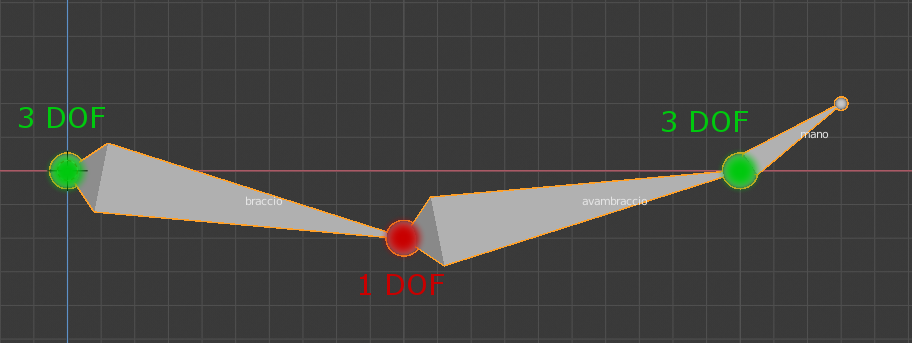
\includegraphics[width=.8\textwidth]{Figures/arm}
\decoRule
\caption[Rig braccio]{Esempio di un semplice rig per il braccio.}
\label{fig:arm}
\end{figure}

Le braccia devono essere in grado di estendersi per raggiungere e afferrare oggetti.
Come spiegato in precedenza (Capitolo \ref{Chapter3}), ha senso fare utilizzo dell'IK per posizionare la mano dove si vuole, e lasciare che il resto del braccio venga posizionato di conseguenza.
In tal caso è opportuno identificare quante articolazioni sono necessarie nel braccio e quanti DOF servono in ciascuna di esse.
Un buon modo di rappresentare gli arti superiori è quello di utilizzare 7 DOF: 3 per la spalla e il polso, 1 per il gomito (vedi Figura \ref{fig:arm}).

Un altro modo è quello di aggiungere un articolazione a metà dell'avambraccio per permettere la rotazione longitudinale di esso.
In altri casi l'avambraccio è staccato dal braccio, questo permette di evitare di dover deformare la mesh, ma il taglio netto tra avambraccio e braccio non sempre è conveniente in termini di visualizzazione.
Per tutte le figure umane nel nostro progetto è stata utilizzata la prima rappresentazione (Figura \ref{fig:arm}).
Nel corto, appaiono anche dei robot, per i quali sarebbe potuto essere utilizzata la terza rappresentazione, più semplice.
È stato tuttavia scelto di utilizzare comunque la prima per permettere di avere lo stesso scheletro per tutti i personaggi, in modo da avere un rig uniforme e non dover fare del lavoro doppio.

Un'ultima considerazione da fare è che ci sono alcuni casi in cui è preferibile poter animare il braccio attraverso FK.
Per questo motivo è stato scelto di utilizzare un rig che permetta di alternare tra FK e IK.
Nel caso della FK è inoltre opportuno rendere la rotazione del braccio indipendente da quella del corpo.
Questa caratteristica è quasi sempre indispensabile, se si pensa ad esempio al ritardo del movimento delle braccia, quando quando le si lascia andare (a peso morto), rispetto a quello del busto, facendolo ruotare a destra e sinistra.
Esistono  però dei casi in cui è preferibile che le braccia mantengano la rotazione del busto, ad esempio nel caso di un robot.
Siccome lo stesso rig verrà utilizzato sia per umani che robot, ha senso far si che questa caratteristica sia attivabile e disattivabile a seconda di chi stia implementando il rig.

\begin{figure}
\centering
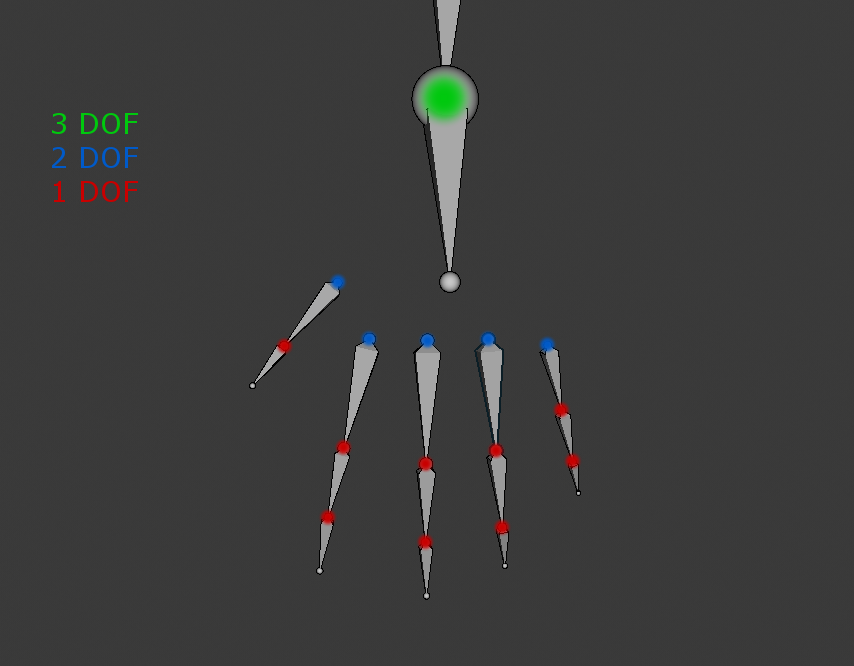
\includegraphics[width=.8\textwidth]{Figures/hand}
\decoRule
\caption[Rig mano]{Esempio di un semplice rig per la mano}
\label{fig:hand}
\end{figure}

\newpage
Per quanto riguarda il rig della mano un modello molto utilizzato è quello rappresentato in Figura \ref{fig:hand}.
In alcuni casi un osso aggiuntivo è presente per ogni dito, tra la falange e il polso, per permettere un maggiore controllo e livello di dettaglio.
Nel nostro caso, questa scelta non è stata ritenuta necessaria, preferendo un rig più semplice e più veloce da animare. 
Un modo più semplice invece, soprattutto usato in videogiochi che utilizzano il minor numero possibile di poligoni, è quello di raggruppare alcune dita.
È molto importante scegliere il giusto bilancio tra livello di controllo e semplicità d'uso, questo trade-off infatti non permette di massimizzare entrambe le caratteristiche.
Siccome per le dita non è necessario avere un IK, non sono necessarie ulteriori progettazioni. Verrà semplicemente usato l'FK per il resto della mano.

Ora che le articolazioni sono state individuate e, per ciascuna di esse, si sa quanti DOF serviranno, è possibile procedere con la scelta della giusta rappresentazione di rotazione (\ref{Section3.1} Rappresentazioni di rotazione).
Basandoci su quanto visto nel Capitolo \ref{Chapter3}, si può dedurre che per le articolazioni con 3 DOF andranno utilizzati dei quaternioni. Mentre per le altre è possibile usare gli angoli di Eulero.

Nel caso di rotazione euleriana è anche necessario scegliere l'ordine degli assi, in base a quelli sui quali verrà effettuata la rotazione:
\begin{itemize}
    \item più usato -> anello (Figura \ref{fig:euler}) esterno, allineato globalmente/osso genitore;
    \item secondo più usato -> anello interno, rotazione locale;
    \item meno usato/non usato -> secondo, causa gimbal lock;
\end{itemize}

\subsection{Arti inferiori}

\begin{figure}
\centering
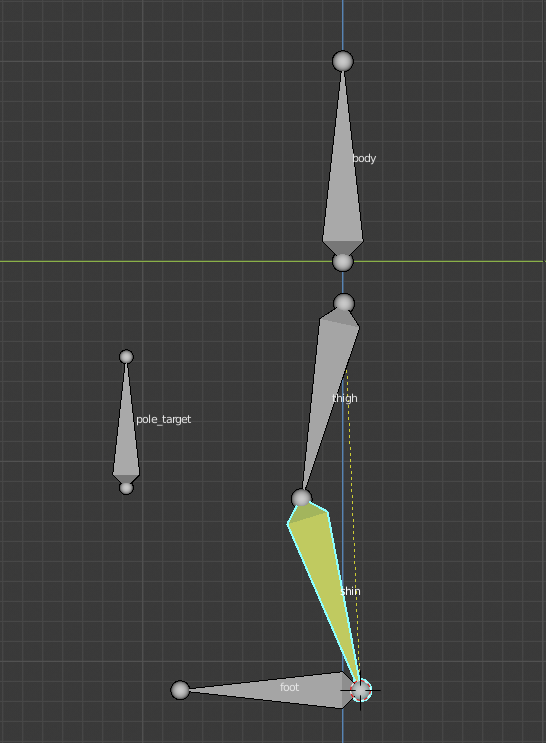
\includegraphics[width=.8\textwidth]{Figures/leg}
\decoRule
\caption[Rig gamba]{Esempio di un semplice rig per la gamba}
\label{fig:leg}
\end{figure}

Per progettare il rig delle gambe in maniera che sia efficacie, bisogna pensare a qual è il modo più conveniente di animare una camminata.

Ad un certo punto il piede poggia a terra e deve rimanere fisso in quella posizione. Il corpo, invece, continua a spostarsi in avanti.
Se usassimo la cinematica diretta, ogni volta che il corpo viene spostato in avanti, dovremmo riposizionare il piede nella posizione in cui era (i.e. counter-animation), in quanto quest'ultimo è discendente del corpo.
In alternativa potremmo rimodellare l'intera gerarchia per far si che il piede si trovi più in alto nella gerarchia rispetto al corpo. Ma questo sarebbe una pessima scelta per ovvi motivi.
Come nell'esempio della mano sulla maniglia, anche qui serve utilizzare una IK, per muovere il resto del corpo indipendentemente dal piede.
Le gambe possono quindi essere controllate interamente attraverso la cinematica inversa (Sezione \ref{sectionIK}).
Siccome questo metodo è sotto-vincolato (i.e. esistono più soluzioni), resta da specificare un vincolo aggiuntivo, relativo all'articolazione intermedia (il ginocchio).

Per fare ciò, è possibile aggiungere un osso, figlio del piede, che servirà per direzionare il ginocchio.
Il motivo per cui, quest'ultimo osso, viene solitamente definito come figlio del piede, è per il semplice motivo che piede e ginocchio puntano solitamente nella stessa direzione.
In questo modo il ginocchio eredita la rotazione del piede, semplificando ulteriormente il lavoro dell'animatore.

In blender questo osso viene chiamato \emph{Pole Target} \cite{blendDoc}, ed il suo funzionamento è molto semplice: tracciando una linea immaginaria dalla base della gamba all'end-effector, viene individuato l'asse che collega i due poli della sequenza delle ossa che costituisce la cinematica inversa.
In Figura \ref{fig:leg} questo asse è rappresentato da una linea tratteggiata gialla.
Ruotando l'intera sequenza di ossa intorno a questo asse, si ottengono infinite soluzioni ammissibili, in cui l'articolazione del ginocchio è l'unica a cambiare posizione, descrivendo una sorta di "equatore" intorno all'asse.
Ora, tracciando un'altra linea, che collega la base del \emph{pole target} all'asse precedentemente menzionato, e perpendicolare a quest'ultimo, avremo un modo di rappresentare la posizione esatta del ginocchio, attraverso l'angolo formato da quest'ultima linea rispetto alla posizione originale.
Si noti che la seconda linea rimane sempre perpendicolare all'asse. Quindi una traslazione del \emph{pole target} parallela all'asse, non ha effetto sulla rotazione della gamba.

In fine, come è stato fatto per il gomito, si può forzare il ginocchio a piegarsi su un singolo asse, garantendo un movimento ancora più realistico in fase di animazione.


 
%% Chapter 5

\chapter{Sviluppo} % Main chapter title

\label{Chapter5} % Change X to a consecutive number; for referencing this chapter elsewhere, use \ref{ChapterX}

%----------------------------------------------------------------------------------------
%	SECTION 1
%----------------------------------------------------------------------------------------

\section{Modellazione}
\begin{itemize}
    \item modelli "lowpoly"
\end{itemize}
\section{Texturing}
\section{Rigging e Animazione}
Rigging è un termine generale che si riferisce all'aggiunta di controlli ad un oggetto, tipicamente allo scopo di animarlo \parencite{blendDoc}.
Consiste nell'assegnare relazioni tra oggetti \parencite{BlendTut}.
\section{Animazione di un corpo umano}
\subsection{Arti superiori}
dita: FK
braccia: mixing FK and IK
\subsection{Arti inferiori}
gambe: IK
\section{Espressioni facciali}
uso di shape keys
ogni vertice è importante, inutile associare un'osso per ogni gruppo di vertici: meglio avere diverse espressioni (set finito) e sciegliere quale si vuole usare in ase ad un valore reale (continuo)

dialoghi
menzionare Rhubarb

divisione dx/sx

Reference
\begin{itemize}
    \item Dialog - The Animator's Survival Kit (p.304) 
    \item Facial animation - Algorithms\&Techniques (p.491)
\end{itemize}
\section{Lighting}
\section{Rendering}

 

%----------------------------------------------------------------------------------------
%	THESIS CONTENT - APPENDICES
%----------------------------------------------------------------------------------------

\appendix % Cue to tell LaTeX that the following "chapters" are Appendices

% Include the appendices of the thesis as separate files from the Appendices folder
% Uncomment the lines as you write the Appendices

% Appendix A

\chapter{Frequently Asked Questions} % Main appendix title

\label{AppendixA} % For referencing this appendix elsewhere, use \ref{AppendixA}

\section{How do I change the colors of links?}

The color of links can be changed to your liking using:

{\small\verb!\hypersetup{urlcolor=red}!}, or

{\small\verb!\hypersetup{citecolor=green}!}, or

{\small\verb!\hypersetup{allcolor=blue}!}.

\noindent If you want to completely hide the links, you can use:

{\small\verb!\hypersetup{allcolors=.}!}, or even better: 

{\small\verb!\hypersetup{hidelinks}!}.

\noindent If you want to have obvious links in the PDF but not the printed text, use:

{\small\verb!\hypersetup{colorlinks=false}!}.

%\include{Appendices/AppendixB}
%\include{Appendices/AppendixC}

%----------------------------------------------------------------------------------------
%	BIBLIOGRAPHY
%----------------------------------------------------------------------------------------

\printbibliography[heading=bibintoc]

%----------------------------------------------------------------------------------------

\end{document}  
